% Author: Giulio Romualdi 
\documentclass[tikz, border=10pt]{standalone}
\usetikzlibrary{arrows}
\begin{document}

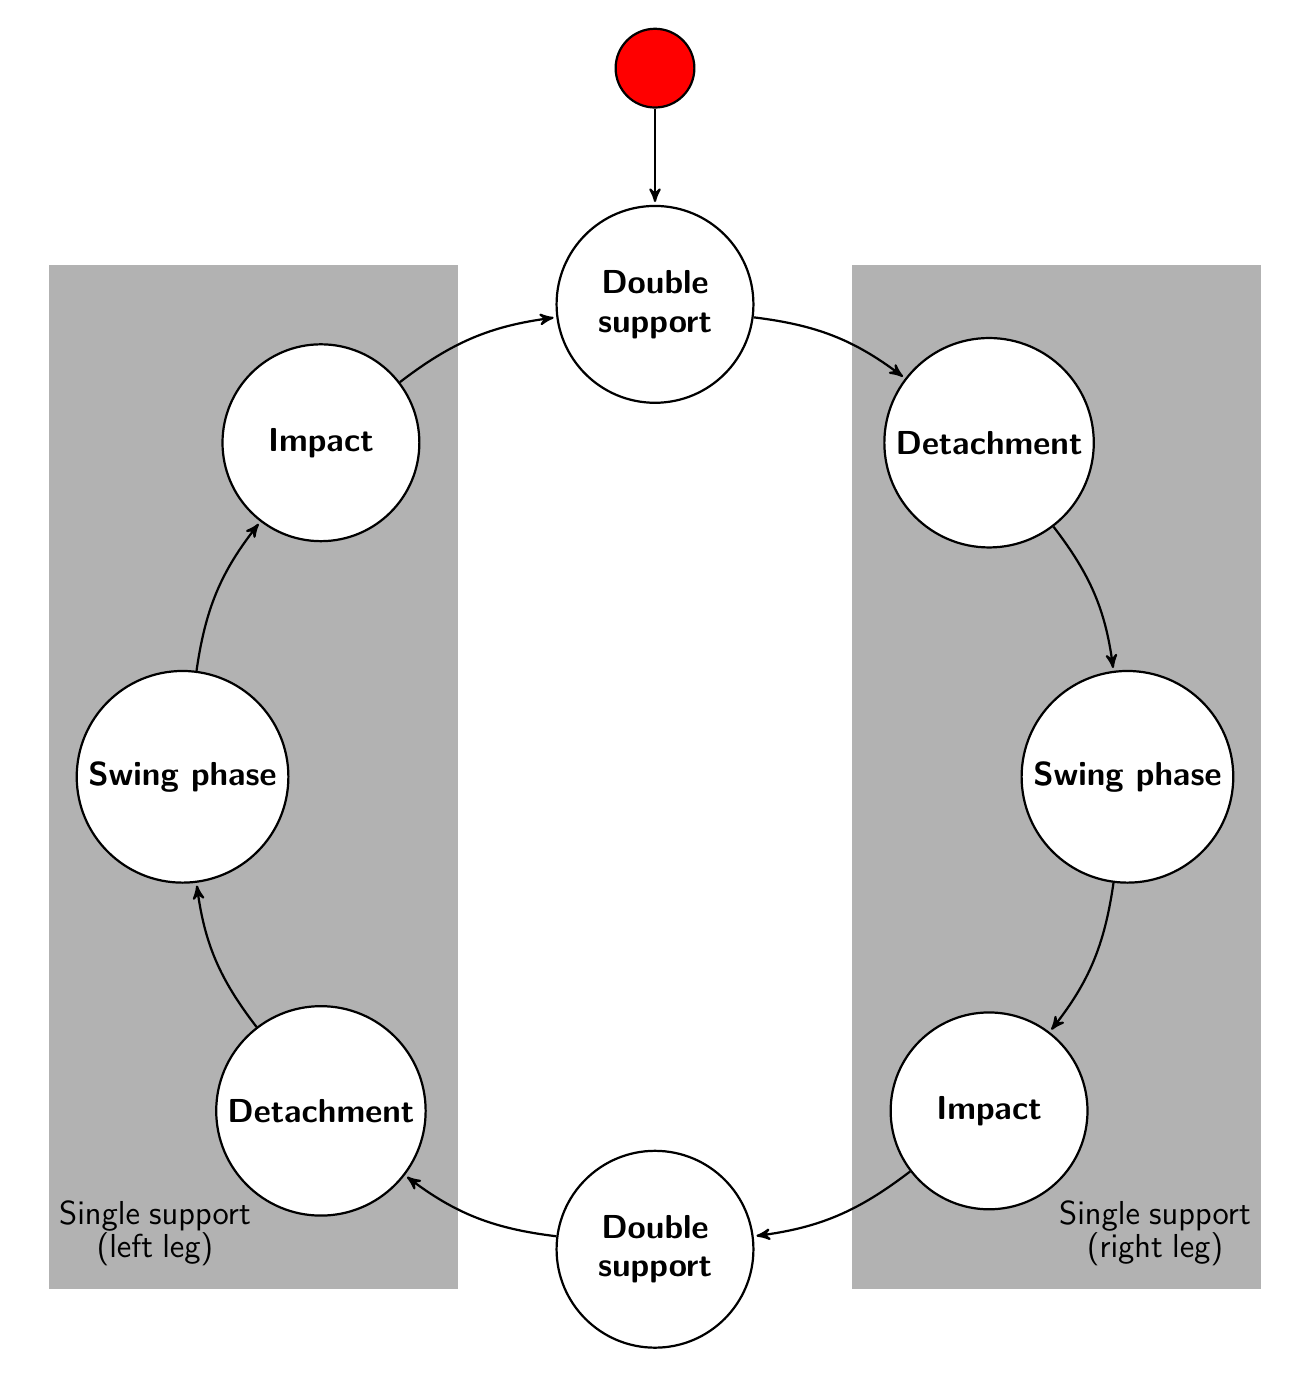
\begin{tikzpicture} [->,>=stealth',shorten >=1pt,auto,node distance=3cm,
    thick,
    doublesupport node/.style={circle,fill=white,align=center,draw,
      font=\sffamily\large\bfseries,minimum size=2.5cm},
    singlesupport node/.style={circle,fill=white,align=center,draw,
      font=\sffamily\large\bfseries,minimum size=2.5cm},
    starting node/.style={circle,fill=red,draw,minimum size=1cm}]

  \fill[color = gray!60] (2.5,6.5) rectangle (7.7,-6.5);
  \fill[color = gray!60] (-2.5,6.5) rectangle (-7.7,-6.5);

  \node[text width=3cm, align=center, font=\sffamily] at (6.35,-5.8){\large Single support\\ (right leg)};
  \node[text width=3cm, align=center, font=\sffamily] at (-6.35,-5.8){\large Single support\\ (left leg)};
  
  
  % draw the nodes of the fsm
  \node [singlesupport node] (swing_r) at (0:6cm) {Swing phase};
  \node [singlesupport node] (detachment_r) at (45:6cm) {Detachment};
  \node [doublesupport node] (ds_1) at (90:6cm) {Double\\support};
  \node [singlesupport node] (impact_l) at (135:6cm) {Impact};
  \node [singlesupport node] (swing_l) at (180:6cm) {Swing phase};
  \node [singlesupport node] (detachment_l) at (225:6cm) {Detachment};
  \node [doublesupport node] (ds_2) at (270:6cm) {Double\\support};
  \node [singlesupport node] (impact_r) at (315:6cm) {Impact};

  \node [starting node, above of = ds_1] (start){};

  % connectors between the nodes
  \draw[->] (start) to (ds_1);
  \draw[->] (ds_1) to [bend left=15] (detachment_r);
  \draw[->] (detachment_r) to [bend left=15] (swing_r);
  \draw[->] (swing_r) to [bend left=15] (impact_r);
  \draw[->] (impact_r) to [bend left=15] (ds_2);
  \draw[->] (ds_2) to [bend left=15] (detachment_l);
  \draw[->] (detachment_l) to [bend left=15] (swing_l);
  \draw[->] (swing_l) to [bend left=15] (impact_l);
  \draw[->] (impact_l) to [bend left=15] (ds_1);
  
\end{tikzpicture}
\end{document}
